\chapter{Testy systemu} \label{chapter_tests}

Jak zaznaczono w celu pracy (\ref{intro_objective}), prototyp systemu
ma być w pełni testowalny. Testy wykonywane są wewnątrz systemu ciągłej integracji 
(\textit{CI/CD}), opisanym w rozdziale \ref{chapter_deployment}. Poniższy rozdział opisuje
rozwiązania zastosowane w celu przetestowania działania systemu,
zanim został on uruchomiony na prawdziwym dronie.

\section{Testy jednostkowe}

Komponenty systemu zaopatrzone są w testy jednostkowe, co pozwala na
sprawdzenie działania kodu w zakresie poszczególnego komponentu.
Przykład testu jednostkowego wykorzystywanego w systemie
zawarty jest w listingu \ref{list:unit_test_example}.

\begin{lstlisting}[
    language=Python,
    label=list:unit_test_example,
    caption={
        Test jednostkowy modułu sterującego uruchamianiem symulatoru drona.
        test sprawdza, czy symulator uruchamia się, oraz czy zostaje poprawnie
        zamknięty po wywołaniu metody \texttt{.stop()}.
    },
    basicstyle=\footnotesize\ttfamily
]
def test_container_lifecycle():
	# Check how many docker containers are running
	num_of_containers = int(check_output('docker ps | wc -l', shell=True))

	print('setting up the runnner')
	runner = SitlDockerHelper('ArduCopter', run_in_background=True)

	print('running the container')
	runner.run()
	sleep(10)

	new_num_of_containers = int(
        check_output('docker ps | wc -l', shell=True)
    )

	# Check if the number of running containers has increased
	assert num_of_containers + 1 == new_num_of_containers

	print('stopping')
	runner.stop()

	# Check if the num of running containers is back to the start state
	assert int(check_output('docker ps | wc -l', shell=True)) == num_of_containers
\end{lstlisting}

Wykonywanie testów w systemie \textit{CI/CD} zwiększa sprawność
pracy z systemami kontroli wersji. W przypadku implementowania nowej 
funkcji na gałęzi (\textit{branch}), system \textit{CI/CD} pozwala określić,
czy nowa funkcjonalność nie destabilizuje systemu -- ostrzegając przed 
przyjęciem na główną gałąź (\textit{master branch}) kodu, który nie przeszedł
testów jednostkowych. Rysunek \ref{failed_pipeline} przedstawia przykład takiego zachowania,
na przykładzie usługi \textit{GitLab}.

\begin{figure}[H]
	\centering
	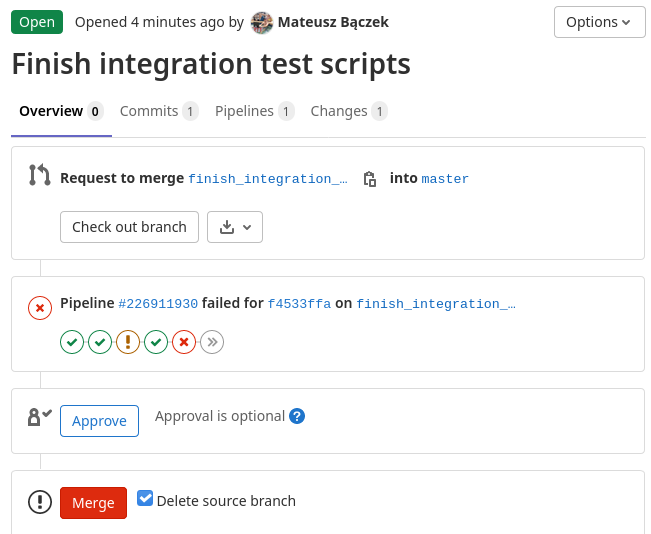
\includegraphics[width=0.8\linewidth]{rys05/failed_pipeline.png}
    \caption{
        Widok interfejsu scalania gałęzi w serwisie \textit{GitLab}.
        Gałąź \texttt{finish\_integration\_tests} nie przechodzi testów
        w systemie \textit{CI/CD}. Administrator repozytorium natychmiast
        ma informację, że kod nie jest jeszcze gotowy do scalenia.
    }
	\label{failed_pipeline}
\end{figure}


\section{Testy integracyjne}

Realizowany w pracy system nie ogranicza się do pojedynczego,
samodzielnego komponentu, zawiera kilka równolegle działających
usług. testy jednostkowe nie są w takim przypadku wystarczające,
aby gruntownie sprawdzić poprawność działania kodu. 

Dodatkowym wyzwaniem przy projektowaniu testów jest interakcja z dronem,
którego kontroler lotu komunikuje się z systemem za pośrednictwem 
interfejsu \texttt{UART}, podłączonego do komputera pokładowego.
Błąd w komunikacji z kontrolerem lotu może doprowadzić do 
rozbicia maszyny, straty są tutaj zupełnie realne, inaczej
niż w przypadku testowania systemów pracujących jedynie na serwerach. 

\subsection{
    Symulacja i symulatory
    \color{white}\cite{simulation_and_simulacra}}

Symulatory lotu są szeroko wykorzystywane w przemyśle lotniczym
\cite{simulation_and_simulators}. Amatorskie otwartoźródłowe kontrolery
lotu nie są tutaj wyjątkiem -- jak wspomniano~w rozdziale poświęconym
kontrolerom lotu (\ref{flight_controller}), wykorzystywane w projekcie 
oprogramowanie \textit{ArduPilot} ma możliwość pracy w trybie SITL
(\textit{software in the loop}). Jest to możliwe dzięki specjalnym opcjom,
które można ustalić w trakcie kompilacji. Opcje umożliwiają przemapowanie
interfejsów kontrolujących peryferia samolotu na ich wirtualne odpowiedniki,
które podłączane są do symulatora. Kod sterujący zachowaniem drona 
oraz dane telemetryczne pozostają takie same jak w przypadku
pracy na prawdziwej maszynie. Szczegółowy diagram 
ilustrujący przemapowywane peryferia kontrolera lotu 
zawarty jest na rysunku~\ref{sitl_diagram}.

\begin{figure}[H]
	\centering
	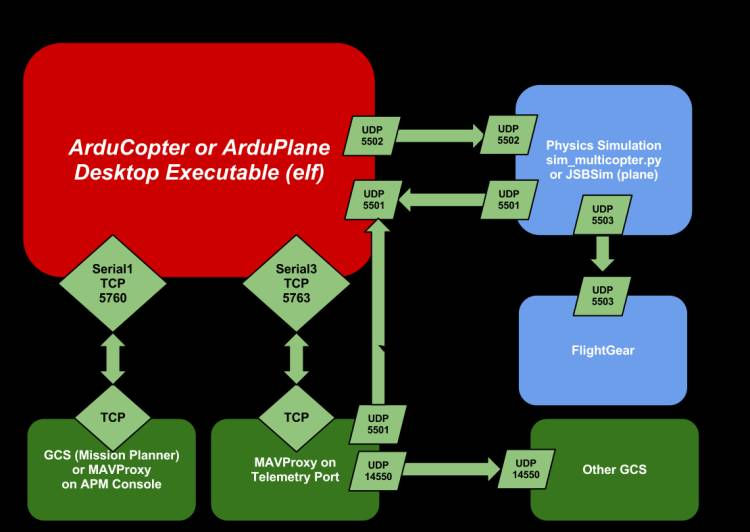
\includegraphics[width=0.9\linewidth]{rys05/sitl.jpg}
    \caption{
        Diagram zaczerpięty z dokumentacji \textit{ArduPilota}
        \cite{ardupilot_sitl}, ilustrujący działanie symulatora SITL.
    }
	\label{sitl_diagram}
\end{figure}





\section{Testy w terenie}

